\newpage

\section{Actividad 2: Polarización de la juntura BE}

\paragraph{Armar el circuito en una plataforma de simulación con el objetivo de observar la curva de la corriente de base a medida que aumenta la tensión de polarización de la juntura base-emisor. Es importante identificar el codo de la corriente y la estabilidad de la tensión VBE una vez polarizada la juntura. Podría, sí le parece, hacer simulaciones modificando otros parámetros que en el circuito básico se encuentran fijos como VCC(V2) o la temperatura ambiente simulada.}



\subsection{Materiales usados:}
\begin{itemize}
    \item Transistor BC546/7/8/9.
    \item Resistores $R_s = \SI{10}{\kilo\ohm}$, $R_c = \SI{560}{\ohm}$.
    \item Fuentes de alimentación.
\end{itemize}


\subsection{Mediciones:}
Mantenemos la $V_{CC} = 10V$, realizamos un barrido de 0V a 10V de $V_{BB}$ para completar la siguiente tabla:

\begin{table}[ht]
\resizebox{\columnwidth}{!}{%
\begin{tabular}{|l|l|l|l|l|l|l|}
\hline
\rowcolor[HTML]{FFFFFF} 
\cellcolor[HTML]{FFCE93}$V_{BB}$ & $500mV$      & $1V$          & $2V$        & $3V$        & $4V$        & $5V$        \\ \hline
\cellcolor[HTML]{FFCE93}$I_B$    & $4,64 \mu A$ & $30,43 \mu A$ & $124 \mu A$ & $220 \mu A$ & $323 \mu A$ & $913 \mu A$ \\ \hline
\cellcolor[HTML]{FFCE93}$V_{BE}$ & $0,493 V$    & $0,682 V$     & $0,73 V$    & $0,74 V$    & $0,74 V$    & $0,75 V$    \\ \hline
\end{tabular}%
}
\end{table}

\begin{figure}[H]
    \centering
    \resizebox{0.49\textwidth}{!}{%
    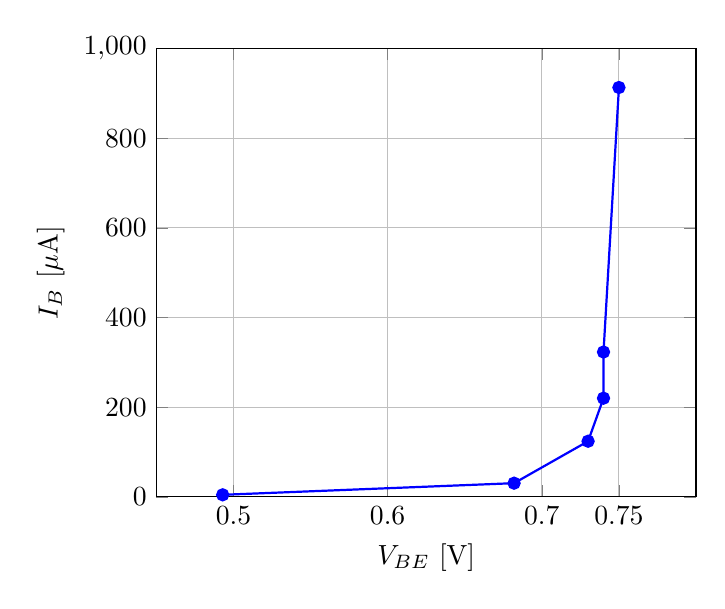
\begin{tikzpicture}
        \begin{axis}[
            xlabel={$V_{BE}$ [V]},
            ylabel={$I_B$ [$\mu$A]},
            grid=both,
            xmin=0.45, xmax=0.8,
            ymin=0, ymax=1000,
            xtick={0.5,0.6,0.7,0.75},
            ytick={0,200,400,600,800,1000},
            legend pos=north west,
        ]
        \addplot[
            color=blue,
            mark=*,
            thick
        ] coordinates {
            (0.493,4.5)
            (0.682,30.43)
            (0.73,124)
            (0.74,220)
            (0.74,323)
            (0.75,913)
        };
        \end{axis}
    \end{tikzpicture}
    }
    \caption{Curva de $I_B$ en función de $V_{BE}$}
    \label{fig:ib_vs_vbe}
\end{figure}
